\begin{samplecase}
{\bf Astrophysical reaction rates : n + ${}^{187}$Os}\newline
With TALYS, astrophysical reaction rates can be calculated.
As sample case, we took the work done in
Ref.\cite{Segawa2007} where the ${}^{187}$Os(n,$\gamma$) was studied for
the derivation of the age of the galaxy withing the
Re-Os cosmochronology. 
\subsubsection{Case a: ${}^{187}$Os(n,$\gamma$) cross section}
First, the calculated ${}^{187}$Os(n,$\gamma$) was compared with experimental data,
using the following input file

\VerbatimInput{\samples n-Os187-astro-ng/org/talys.inp}

The results are given in Fig.\ref{os187ng}.
\subsubsection{Case b: ${}^{187}$Os(n,$\gamma$) astrophysical reaction rate}
Next, the astrophysical reaction rates for neutrons on ${}^{187}$Os are computed 
with the following input file

\VerbatimInput{\samples n-Os187-astro-rate/org/talys.inp}

which produces various output files in which the reaction rates as 
function of temperature are given.
The $(n,\gamma )$ rate as given in the output file is   
{\small \begin{verbatim}

 8. Thermonuclear reaction rates                                                 
 Reaction rate for Z= 76 A=188 (188Os)                                           
    T        G(T)        Rate            
   0.0001 1.00000E+00 5.46242E+08                                                  
   0.0005 1.00000E+00 4.96512E+08
   0.0010 1.00000E+00 4.45882E+08                                                  
   0.0050 1.00000E+00 3.52813E+08
   0.0100 1.00002E+00 3.01755E+08                                                  
   0.0500 1.20827E+00 2.03467E+08
   0.1000 1.64630E+00 1.87256E+08                                                  
   0.1500 1.95860E+00 1.82416E+08
   0.2000 2.21894E+00 1.80436E+08                                                  
   0.2500 2.48838E+00 1.79690E+08
   0.3000 2.79031E+00 1.79474E+08                                                  
   0.4000 3.49874E+00 1.79716E+08
   0.5000 4.31540E+00 1.80165E+08
   0.6000 5.20597E+00 1.80375E+08
   0.7000 6.15215E+00 1.80187E+08
   0.8000 7.14759E+00 1.79580E+08
   0.9000 8.19300E+00 1.78579E+08
   1.0000 9.29313E+00 1.77221E+08
.....................................
\end{verbatim} } \renewcommand{\baselinestretch}{1.07}\small\normalsize
\noindent
The same numbers can be found in the separate file {\em astrorate.g}.
In {\em astrorate.tot} the rates for all reactions can be found.

\end{samplecase}
\begin{figure}
\centering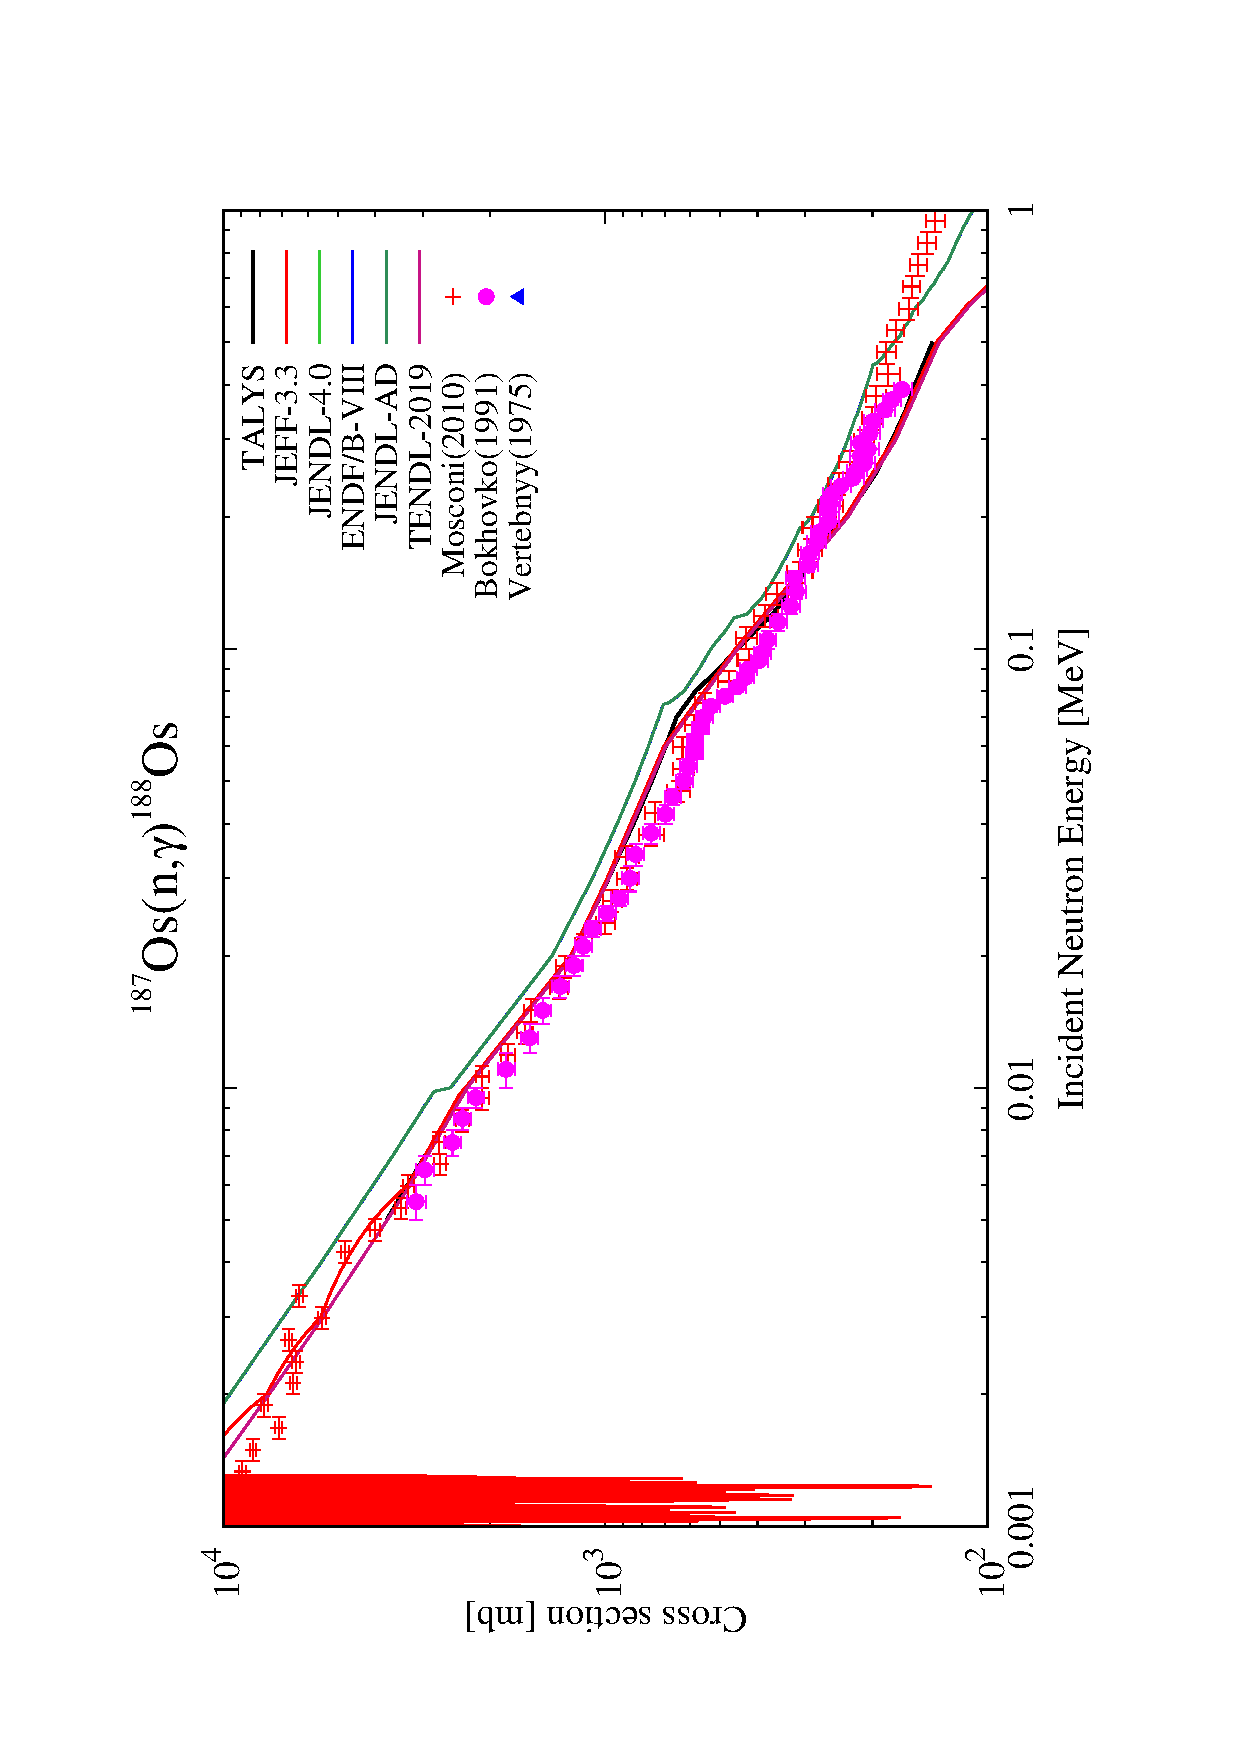
\includegraphics[scale=0.5,angle=270]{n-Os187-ng}
\caption{${}^{187}$Os(n,$\gamma$) cross section.}
\label{os187ng}
\end{figure}
